\graphicspath{{images/}}

\subsection{Численные методы решения ДУЧП гиперболического типа}

\subsubsection{Постановка задачи}
Используя явную схему крест и неявную схему, решить начально-краевую задачу для дифференциального уравнения гиперболического типа. Аппроксимацию второго начального условия произвести с первым и со вторым порядком. Осуществить реализацию трех вариантов аппроксимации граничных условий, содержащих производные: двухточечная аппроксимация с первым порядком, трехточечная аппроксимация со вторым порядком, двухточечная аппроксимация со вторым порядком. В различные моменты времени вычислить погрешность численного решения путем сравнения результатов с приведенным в задании аналитическим решением $U(x, t)$. Исследовать зависимость погрешности от сеточных параметров $\tau$, $h$.

\subsubsection{Вариант 9}
$$ {{\partial^2 u} \over {\partial t^2}} = {{\partial^2 u} \over {\partial x^2}} + 2 \cdot {{\partial u} \over {\partial y}} - 3 \cdot u - 2 \cdot {{\partial u} \over {\partial t}} $$
$$ u(0, t) = e ^ {-t} \cdot \cos(2t) $$
$$ u({{\pi} \over {2}}, t) = 0 $$
$$ u(x, 0) = e ^ {-x} \cdot \cos{x} $$
$$ u'_t(x, 0) = -e ^ {-x} \cdot \cos{x} $$
Аналитическое решение:
$$ U(x, t) = e ^ {-t-x} \cdot \cos{x} \cdot \cos(2t) $$
\pagebreak

\subsubsection{Результат}
\begin{center}
    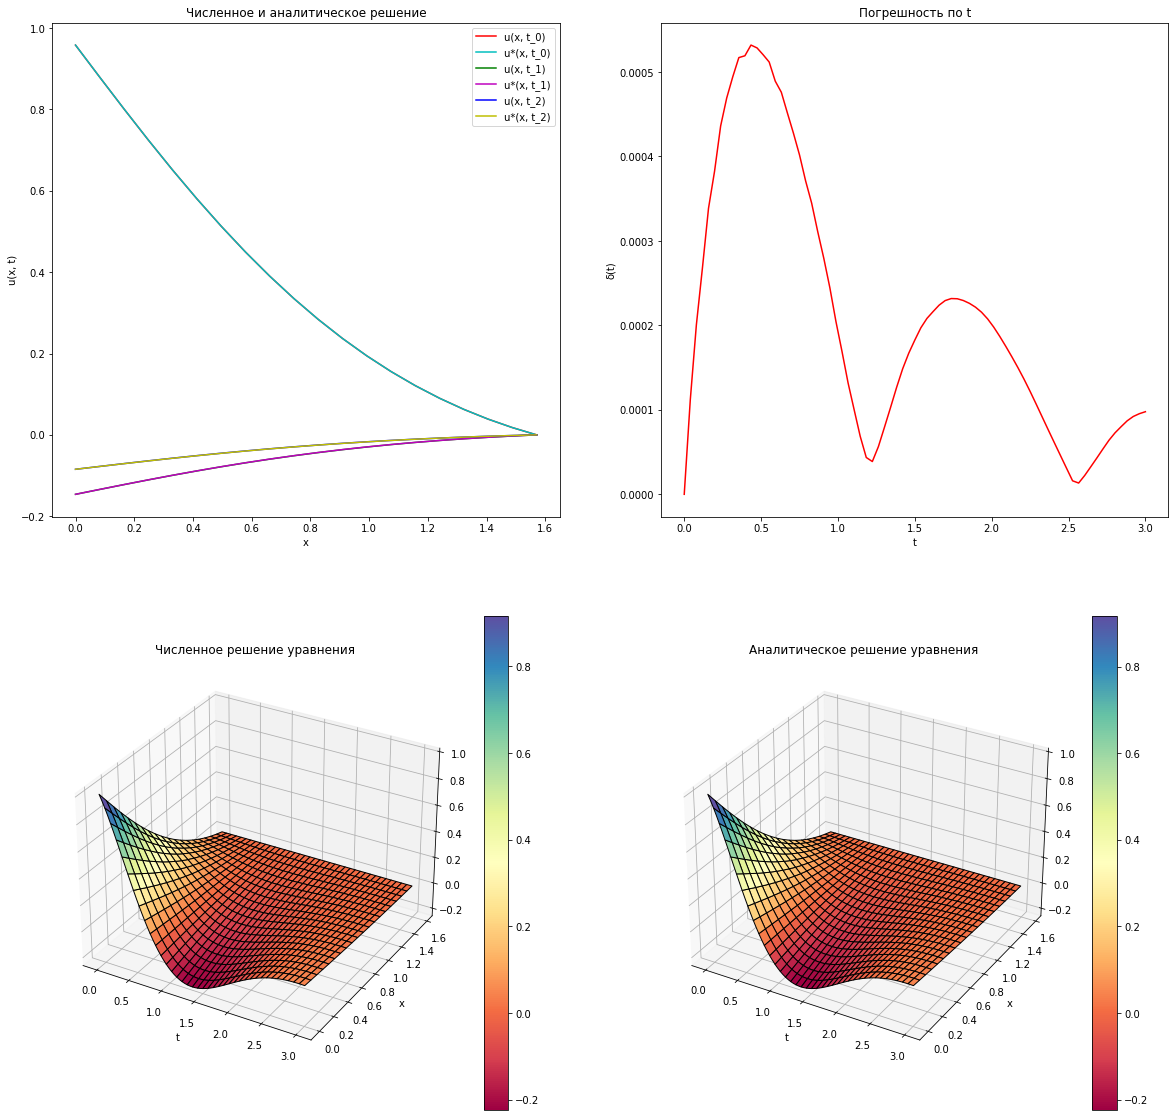
\includegraphics[width=\textwidth]{6.png}\newline\noindent
\end{center}
\pagebreak

\subsubsection{Исходный код}
\lstinputlisting{../lab6/hpde.hpp}
\pagebreak
